\documentclass[11pt,a4paper]{article}

% ---------- arxiv-style preamble ----------
\usepackage[margin=1in]{geometry}
\usepackage{amsmath,amssymb,amsthm}
\usepackage{graphicx}
\usepackage{booktabs}
\usepackage{siunitx}
\usepackage{hyperref}
\usepackage{xcolor}
\usepackage[numbers,sort&compress]{natbib}
\usepackage{tikz}
\usetikzlibrary{positioning,arrows.meta}
\usepackage{pgfplots}
\pgfplotsset{compat=1.18}
\usepgfplotslibrary{groupplots}
\usepackage{caption}
\usepackage{listings}
\usepackage{array}
\captionsetup{font=small,labelfont=bf}
\hypersetup{
  colorlinks=true,
  linkcolor=blue!50!black,
  citecolor=blue!50!black,
  urlcolor=blue!50!black
}

% ---------- emoji tier badges ----------
\providecommand{\tierBlue}{🔵}
\providecommand{\tierGreen}{🟢}
\providecommand{\tierYellow}{🟡}
\providecommand{\tierOrange}{🟠}
\providecommand{\tierRed}{🔴}

\newcommand{\bigphi}{\ensuremath{\Phi}}

\title{
  \textbf{Integrated Information Tracks Inter-Element Flow, Not Single-System Entropy}\\[4pt]
  \large A three-measure triangulation of faithful IIT~4.0 \bigphi{} against
  Shannon entropy, Lempel--Ziv complexity, and transfer entropy on
  cellular-automaton substrates
}

\author{
  \texttt{anima} maintainers\\
  \normalsize\textit{dancinlab}\\[2pt]
  \normalsize\href{https://github.com/dancinlab/anima}{\texttt{github.com/dancinlab/anima}}
}

\date{\today}

\begin{document}

\maketitle

% =========================================================================
\begin{abstract}
Integrated Information Theory (IIT) claims that integrated information
\bigphi{} is \emph{not} the same quantity as classical information. We test
this on the theory's own causal engine by triangulating faithful IIT~4.0
big-\bigphi{} against three classical information measures on an identical
ten-rule elementary-cellular-automaton (ECA) panel: Shannon output entropy,
Lempel--Ziv (LZ76) algorithmic complexity, and transfer entropy. The
measures dissociate sharply. \bigphi{} is \emph{orthogonal} to Shannon
entropy (Pearson \(r=0.36\)): the identity rule carries maximal output
entropy (\SI{4}{bit}) yet has \bigphi{}=0, while the most-integrated rule has
sub-maximal entropy. \bigphi{} \emph{aligns} with LZ complexity (\(r=0.83\),
Spearman \(\rho=0.94\)) and, most strongly, with transfer entropy
(\(r=0.88\), \(\rho=0.82\)). Yet every classical measure has a blind spot
that \bigphi{} does not: LZ over-predicts on self-similar dynamics
(rule~90, \bigphi{}=0), and bivariate transfer entropy under-predicts on
synergistic XOR coupling (rules~150/105, \bigphi{}\(>0\) yet TE\(=0\)).
A multivariate transfer entropy recovers the XOR synergy but does
\emph{not} improve the fit --- the correlation drops to \(r=0.71\) because
it now over-counts non-integrated flow (rule~90 again) --- so \emph{no
order} of transfer entropy equals \bigphi{}: one failure mode is traded for
another. A complementary structural experiment shows that at matched edge count a
hub network integrates ($\bigphi=6.81$) where a regular cycle does not
($\bigphi=0$): \bigphi{} is governed by how elements \emph{relate}, not by
how much information or density a system carries. We frame the
Shannon-entropy result as a closed negative confirming IIT's foundational
distinction; we do not claim \bigphi{} equals any classical measure, nor do
we make phenomenal claims. All runs are deterministic, \$0, hexa-native, and
GPU-free; bit-for-bit reproduction records are in \texttt{companion/}.
\end{abstract}

\begin{figure}[h]
\centering
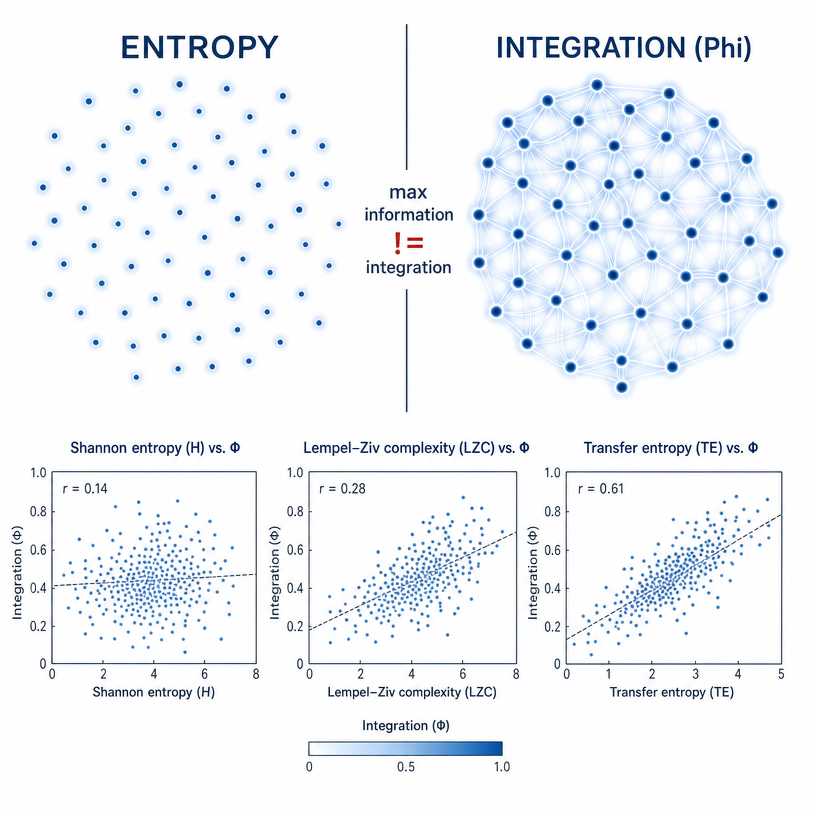
\includegraphics[width=0.62\linewidth]{figures/fig00_cover.png}
\caption{The thesis in one image: the \emph{same} number of bits gives
maximal entropy when scattered (left) but zero integration; woven into a
network (right) the integration \(\bigphi\) is high. \(\bigphi\) is a
property of how elements relate, not of how much information is present.
Conceptual illustration (fal.ai / \texttt{gpt-image}).}
\label{fig:cover}
\end{figure}

\section{Introduction}
\label{sec:intro}

A recurring objection to Integrated Information Theory (IIT)
\citep{tononi2016,oizumi2014} is that its central quantity, integrated
information \bigphi{}, is at bottom a relabelling of classical
information --- that a system with more bits, or more algorithmic
complexity, is simply ``more integrated.'' IIT explicitly denies this:
a pile of \(N\) independent random bits has maximal entropy yet zero
integration, because no partition destroys anything. The claim is
testable, but it is rarely tested \emph{directly} on a causal engine that
can compute \bigphi{} exactly --- correlational proxies for \bigphi{}
cannot cleanly construct ``information without integration.''

We do exactly that. Using a faithful, deterministic IIT~4.0
cause--effect engine, we measure exact state-averaged big-\bigphi{} on a
fixed ten-rule ECA panel and ask, on the \emph{identical} substrates, how
\bigphi{} co-varies with three of the most widely used classical
information measures: Shannon entropy (statistical information),
Lempel--Ziv complexity (algorithmic information~\citep{lempelziv1976}),
and transfer entropy (directed information flow~\citep{schreiber2000}).
Because the substrate and the engine are held fixed, any difference
between the three correlations is attributable to \emph{what each measure
counts}, not to confounds in the system.

\medskip
\noindent\textbf{Contributions.}
\begin{enumerate}\itemsep0.3em
\item A \emph{closed negative} (\tierRed): faithful big-\bigphi{} does not
reduce to Shannon entropy (\(r=0.36\)), witnessed by a max-entropy /
zero-\bigphi{} substrate and a max-\bigphi{} / sub-max-entropy substrate
on the same panel (\S\ref{sec:shannon}).
\item Two positive alignments (\tierGreen): \bigphi{} tracks LZ complexity
(\(r=0.83\)) and transfer entropy (\(r=0.88\)) --- the \emph{inter-element}
measures --- but each has a blind spot \bigphi{} lacks: LZ over-predicts on
self-similar rule~90, bivariate TE under-predicts on synergistic XOR
(\S\ref{sec:lz}--\S\ref{sec:te}).
\item A structural corollary (\tierGreen): at matched edge count, topology
not density governs \bigphi{} (hub \(6.81\) vs.\ cycle \(0\);
\S\ref{sec:structure}). Together: \bigphi{} measures how elements relate.
\item A fully deterministic, GPU-free, \$0 hexa-native pipeline with
pre-registered falsifiers and bit-for-bit companion records
(\S\ref{sec:repro}).
\end{enumerate}

\section{Background}
\label{sec:bg}

\textbf{Faithful IIT~4.0 \bigphi{}.} For a system with a state-by-node
transition probability matrix (TPM), IIT~4.0~\citep{albantakis2023}
defines integrated information by the minimum-information partition (MIP):
the system's cause--effect structure is compared against its value under
the partition that least changes it. We use a deterministic engine that
computes the structure-cut big-\bigphi{} exactly for small \(N\); an ECA
on a periodic ring \emph{is} a TPM, because each cell's next value is a
deterministic function of its three-cell neighbourhood, so the
\(2^N\) states map deterministically to per-cell next values.

\textbf{Three classical measures.}
\emph{Shannon entropy} \(H\) of the output-state distribution under a
uniform input ensemble measures how much information the dynamics
preserve: a bijection preserves all \(N\) bits (\(H=N\)), a constant map
destroys them (\(H=0\)). \emph{Lempel--Ziv} complexity~\citep{lempelziv1976}
of the space--time diagram estimates Kolmogorov (algorithmic) complexity ---
how incompressible the behaviour is. \emph{Transfer entropy}
\citep{schreiber2000} \(\mathrm{TE}(j\!\to\!i)\) measures how much source
cell \(j\)'s present reduces uncertainty about cell \(i\)'s future
\emph{beyond} \(i\)'s own present --- directed, pairwise information flow.
The first is a single-system quantity; the latter two are
inter-element / structural. The synergy literature
\citep{williamsbeer2010} predicts that bivariate transfer entropy is
blind to purely synergistic coupling (e.g.\ XOR), a prediction we
recover empirically.

\section{Related work}
\label{sec:related}

\textbf{\bigphi{} and its proxies.} Because exact \bigphi{} is
super-exponential in \(N\), most empirical work uses proxies ---
perturbational complexity (PCI), Lempel--Ziv of EEG, or correlational
mutual-information surrogates. These proxies cannot \emph{construct}
information-without-integration, because a correlational surrogate of
\bigphi{} inherits whatever the data's information content is; the
dissociation we report (identity rule: max entropy, zero \bigphi{})
requires an engine that computes the causal MIP directly, which is why we
use a faithful IIT~4.0 implementation at small \(N\) rather than a proxy.

\textbf{Cellular-automaton complexity.} Wolfram's classification
\citep{wolfram1984} orders ECA rules by dynamical behaviour (fixed,
periodic, chaotic, complex); LZ complexity of the space--time diagram is a
standard quantitative stand-in for that ordering. Our LZ results recover
the expected ordering (constants low, rule~30 highest), and the LZ--\bigphi{}
alignment shows that dynamical complexity and causal integration largely
co-vary on this family --- with the rule~90 exception precisely where
self-similarity inflates LZ without inflating integration.

\textbf{Information flow and synergy.} Transfer entropy
\citep{schreiber2000} is the standard directed-flow measure; the partial
information decomposition \citep{williamsbeer2010} formalises why pairwise
measures miss synergy. Our XOR result is a minimal, exact instance of that
gap, measured against an independent \bigphi{} ground truth rather than
inferred. To our knowledge the three measures have not previously been
triangulated against \emph{exact} \bigphi{} on one fixed substrate panel
with pre-registered falsifiers.

% =========================================================================
\section{Full Pipeline}
\label{sec:pipeline}

Each experiment runs the same path from a pre-registered question to a
persisted, re-verifiable result. Stages are tier-tagged under the rubric
below; the backing atom is the record that makes the stage independently
re-checkable.

\medskip
\noindent\fbox{\parbox{0.97\linewidth}{\small\textbf{Tier rubric.}
\tierBlue\ closed-form identity \(\cdot\)
\tierGreen\ numerical (reproducible script + persisted output) \(\cdot\)
\tierYellow\ cited (DOI / arxiv) \(\cdot\)
\tierOrange\ install-gated \(\cdot\)
\tierRed\ falsified / closed negative (kept, never deleted).}}

\medskip
\begin{table}[h]
\centering
\small
\begin{tabular}{@{}>{\centering\arraybackslash}m{0.4cm} >{\raggedright\arraybackslash}m{4.6cm} c >{\raggedright\arraybackslash}m{5.6cm}@{}}
\toprule
\textbf{\#} & \textbf{Stage} & \textbf{Tier} & \textbf{Backing atom} \\
\midrule
\textcircled{\scriptsize 1} & Question + frozen falsifiers  & \tierBlue   & \texttt{H\_287..293} pre-register headers \\
\textcircled{\scriptsize 2} & IIT / information background  & \tierYellow & \texttt{references.bib} \\
\textcircled{\scriptsize 3} & Engine anchors (204, 0 \(\to\bigphi{=}0\)) & \tierBlue   & hand-derivable, machine-precision \\
\textcircled{\scriptsize 4} & Per-rule measurement          & \tierGreen  & \texttt{companion/verify-ledger.json} \\
\textcircled{\scriptsize 5} & Correlation \(+\) falsifier sweep & \tierGreen  & \texttt{companion/verify-ledger.json} \\
\textcircled{\scriptsize 6} & Shannon reductive null        & \tierRed    & closed negative (\S\ref{sec:shannon}) \\
\textcircled{\scriptsize 7} & Interpretation                & \tierOrange & speculation-fenced (\S\ref{sec:verify}) \\
\bottomrule
\end{tabular}
\caption{Pipeline stages, each tier-tagged. Exact arithmetic and engine
anchors are \tierBlue/\tierGreen; the empirical reading of ``\bigphi{} is
not entropy'' is honestly held at \tierOrange{} (fenced), never promoted to
a closed-form identity.}
\label{tab:pipeline}
\end{table}

\section{Method}
\label{sec:method}

\textbf{Substrate panel.} Ten elementary CA rules on a periodic ring,
fixed before measurement and held identical across all experiments:
constants \(\{0,255\}\); bijections \(\{204\text{ (identity)},
51\text{ (complement)}\}\); XOR-feedback integrators \(\{150,105\}\);
partial-feedback \(\{90,60\}\); and universal/chaotic rules \(\{110,30\}\).

\textbf{Metrics.} For each rule: (i) big-\bigphi{} is the mean over all
\(2^N\) states of the faithful IIT~4.0 big-\bigphi{} (\(N=4\) exact);
(ii) Shannon output entropy \(H_\mathrm{out}=-\sum_o p(o)\log_2 p(o)\)
over the uniform input ensemble; (iii) normalised LZ76 complexity of the
space--time diagram (ring of \(14\) cells, \(64\) steps, single centre
seed, normalised \(c\log_2 L/L\)); (iv) total transfer entropy
\(\mathrm{TE}_\mathrm{total}=\sum_{i}\sum_{j\neq i}\mathrm{TE}(j\!\to\!i)\),
lag-1 bivariate, over the uniform ensemble.

\textbf{Correlation.} Pearson \(r\) and Spearman \(\rho\) of each measure
against big-\bigphi{} across the ten rules. A reductive seed hypothesis
``\bigphi{} co-varies with measure \(M\)'' is \emph{supported} iff
\(r\ge0.5\), \emph{falsified} otherwise --- a threshold fixed before
measurement (the companion ledger records the frozen falsifiers verbatim).

\textbf{Structure experiment (\S\ref{sec:structure}).} A separate
parity-network generalisation of the ECA$\to$TPM bridge: each node
updates to the XOR of its graph neighbours. We compare a scale-free hub
and a regular cycle at matched edge count, plus empty and complete
anchors.

\textbf{Determinism.} Every experiment is deterministic (no RNG), runs in
\$0 on a laptop CPU, uses no GPU and no language model, and re-runs
bit-for-bit identically. Each was pre-registered with \(\ge3\) falsifiers
frozen before the headline values were read.

\subsection{Formal definitions}
\label{sec:formal}

\textbf{ECA \(\to\) TPM.} For Wolfram rule \(R\in[0,255]\) on a periodic
ring of \(N\) cells, the state-by-node transition matrix entry is
\(\mathrm{TPM}[s,i]=\mathrm{bit}_{4l+2c+r}(R)\), where \((l,c,r)\) are the
left/centre/right neighbours of cell \(i\) in state \(s\). Determinism
makes every entry \(0\) or \(1\); the \(2^N\) states tile the TPM exactly.

\textbf{Big-\bigphi{}.} For state \(s\), the engine computes the IIT~4.0
cause--effect structure and its value under the minimum-information
partition (MIP); big-\bigphi{}(s) is the irreducibility of the structure
under the system cut. We report
\(\bigphi_\mathrm{mean}=2^{-N}\sum_{s}\bigphi(s)\). Two hand-derivable
anchors fix faithfulness: rule~204 (identity, \(\mathrm{next}_i=c\); each
cell self-determined, fully reducible) \(\Rightarrow\bigphi=0\); rule~0
(constant) \(\Rightarrow\bigphi=0\).

\textbf{Shannon output entropy.} Under a uniform input ensemble, let
\(o(s)=\sum_i \mathrm{TPM}[s,i]\,2^i\) be the output state. Then
\(H_\mathrm{out}=-\sum_o p(o)\log_2 p(o)\), with \(p(o)=2^{-N}\,
|\{s:o(s)=o\}|\). A bijection (e.g.\ identity) preserves all \(N\) bits,
\(H_\mathrm{out}=N\); a constant map gives \(H_\mathrm{out}=0\).

\textbf{Lempel--Ziv complexity.} Evolve the rule from a single centre seed
on a ring of \(N_L=14\) cells for \(T=64\) steps; concatenate the
space--time diagram row-major into a length-\(L=N_L T\) binary string and
parse it with the Lempel--Ziv (1976) production rule into \(c\) distinct
phrases. We report \(\mathrm{LZ}_\mathrm{norm}=c\log_2 L / L\), which
\(\to 1\) for a random string.

\textbf{Transfer entropy.} For ordered cell pair \((j\!\to\!i)\), with
\(i'\) the next value of \(i\),
\[
\mathrm{TE}(j\!\to\!i)=\sum_{i',i,j} p(i',i,j)\,
\log_2\frac{p(i'\mid i,j)}{p(i'\mid i)},
\]
estimated over the uniform ensemble (lag-1, bivariate), and
\(\mathrm{TE}_\mathrm{total}=\sum_{i}\sum_{j\neq i}\mathrm{TE}(j\!\to\!i)\).
Bivariate TE conditions only on the target's own present, so a purely
synergistic update (XOR of $\ge2$ sources) leaves
\(p(i'\mid i,j)=p(i'\mid i)\) and contributes zero --- the blind spot of
\S\ref{sec:te}, anticipated by partial-information decomposition
\citep{williamsbeer2010}.

\section{Verify}
\label{sec:verify}

The IIT~4.0 engine reproduces two hand-derivable anchors exactly, fixing
the measurement's faithfulness before any correlation is read: the
identity rule~204 (each cell self-determined, reducible) gives
big-\bigphi{}=0, and the constant rule~0 (no causal power) gives
big-\bigphi{}=0. Both hold to machine precision across all states. The
numerical big-\bigphi{}, entropy, LZ and TE values are deterministic
arithmetic and converge bit-for-bit across fresh process invocations
(falsifier F\(\ast\).DETERMINISM, all four experiments). The empirical
\emph{interpretations} (e.g.\ ``\bigphi{} is not Shannon entropy'') are
not closed-form atlas identities and are therefore honestly
speculation-fenced under the project's verification rubric:

\begin{lstlisting}[basicstyle=\ttfamily\footnotesize,frame=single,xleftmargin=0pt,breaklines=true]
$ hexa verify --fence "faithful IIT4 big-Phi does NOT reduce to Shannon
  entropy across a 10-rule ECA panel (Pearson r=0.363<0.5); identity rule
  204 has MAX output-entropy (4 bit) yet ZERO integration"
=> VERDICT: (white-circle) SPECULATION-FENCED
   reason = deterministic toy-substrate outcome; values are exact
   arithmetic, only the empirical interpretation is fenced (NOT an
   atlas identity)
\end{lstlisting}

\noindent The per-experiment gate counts (anchors $+$ bounds $+$
determinism) are \(11/11\), \(9/9\), \(8/8\) for the three measures and
\(4/4\) for the structure experiment; full breakdown in
\texttt{companion/verify-ledger.json}.

\section{Results}
\label{sec:results}

\subsection{Shannon entropy is orthogonal to \bigphi{} (\tierRed{} closed negative)}
\label{sec:shannon}

Across the panel, big-\bigphi{} does \emph{not} co-vary with Shannon
output entropy: Pearson \(r=0.363<0.5\), so the reductive hypothesis is
falsified. The mechanism is a double dissociation (Tab.~\ref{tab:panel},
Fig.~\ref{fig:headline}, left). The identity rule~204 and complement
rule~51 are bijections: they carry \emph{maximal} output entropy
(\SI{4}{bit}) yet have \bigphi{}=0, because their cells are causally
independent --- maximal information, zero integration. Conversely the
most-integrated rule~60 (\(\bigphi=13.6\)) has \emph{sub-maximal} entropy
(\SI{3}{bit}). At fixed \(H_\mathrm{out}=\SI{4}{bit}\), \bigphi{} ranges
from \(0\) (rule~204) to \(5.6\) (rule~150): no monotone map from entropy
to \bigphi{} can exist. Information is necessary but not sufficient for
integration --- IIT's foundational distinction, confirmed on its own
substrate.

\subsection{Algorithmic (LZ) complexity tracks \bigphi{} (\tierGreen)}
\label{sec:lz}

The other classical currency --- algorithmic complexity, estimated by
LZ76 of the space--time diagram --- \emph{does} track \bigphi{}: Pearson
\(r=0.831\), Spearman \(\rho=0.936\) (Fig.~\ref{fig:headline}, centre).
Constants and identity sit at low LZ / zero \bigphi{}; integrating and
chaotic rules rise together to high LZ / high \bigphi{}. The contrast
with \S\ref{sec:shannon} is the point: on the identical panel, statistical
information is orthogonal to \bigphi{} while algorithmic complexity aligns
with it. The alignment is imperfect, and the imperfection is
diagnostic --- rule~90 (the Sierpi\'nski/XOR-pair rule) has non-trivial LZ
(\(0.24\)) from its self-similar fractal pattern yet \bigphi{}=0: LZ
\emph{over-predicts} integration for self-similar dynamics. LZ is a strong
correlate, not a sufficient condition.

\subsection{Transfer entropy tracks \bigphi{} most strongly --- with a synergy blind spot (\tierGreen)}
\label{sec:te}

Transfer entropy, the directed inter-element measure, is the strongest
correlate: Pearson \(r=0.883\), Spearman \(\rho=0.822\)
(Fig.~\ref{fig:headline}, right). Constants, identity and complement all
have \(\mathrm{TE}_\mathrm{total}=0\) (no inter-cell flow) and
\bigphi{}=0; the integrating/chaotic rules carry both flow and \bigphi{}.
But bivariate TE has a clean blind spot exactly where the synergy
literature predicts one: the pure-XOR integrators rules~150/105 have
\(\bigphi=5.6\) yet \(\mathrm{TE}_\mathrm{total}=0\). XOR integration is
synergistic --- knowing one source's present tells you nothing about a
cell's future beyond the cell's own present --- so it is invisible to
pairwise TE conditioned only on the target's own past.

\subsection{No order of transfer entropy equals \bigphi{} (\tierGreen)}
\label{sec:teorder}

The natural fix for the synergy blind spot is a \emph{multivariate} /
conditional transfer entropy. We measured it directly: for each cell,
\(\mathrm{TEm}_i = H(\mathrm{next}_i \mid \mathrm{self}_i)\), the directed
information from all of \(i\)'s other inputs jointly, beyond \(i\)'s own
present (Tab.~\ref{tab:teorder}). It does recover the synergy --- rules
150/105 jump from \(\mathrm{TE}=0\) to \(\mathrm{TEm}=\SI{4}{bit}\), and the
identity rule stays at \(0\). But it does \emph{not} track \bigphi{} better:
the correlation \emph{drops} from the bivariate \(r=0.883\) to \(r=0.705\)
(\(\rho=0.68\)). The reason is a new, opposite error --- rule~90 receives
flow from its neighbours (\(\mathrm{TEm}=\SI{4}{bit}\)) but is reducible, so
\(\bigphi=0\): multivariate TE \emph{over}-counts non-integrated flow on
exactly the rule where LZ also over-predicted (\S\ref{sec:lz}). So no order
of classical transfer entropy equals \bigphi{}: the bivariate measure
under-counts synergy (rules 150/105), the multivariate measure over-counts
non-integrated flow (rule~90). Recovering the missing synergy does not buy
a better \bigphi{} proxy; it trades one failure mode for another. \bigphi{},
computed over the full cause--effect structure rather than any fixed-order
flow statistic, is subject to neither --- which is the strongest single
statement of the paper's thesis.

\begin{table}[h]
\centering
\small
\begin{tabular}{r ccc}
\toprule
\textbf{rule} & \textbf{bivariate TE} & \textbf{multivariate TEm} & \(\bigphi_\mathrm{mean}\) \\
\midrule
150 (XOR$_3$) & 0.00 & \textbf{4.00} & 5.625 \\
105 (XNOR)    & 0.00 & \textbf{4.00} & 5.625 \\
90  (Sierp.)  & 0.00 & \textbf{4.00} & \textbf{0.000} \\
60            & 4.00 & 4.00 & 13.625 \\
110           & 3.245 & 3.623 & 13.130 \\
30            & 2.00 & 4.00 & 13.885 \\
\midrule
\multicolumn{1}{r}{\textbf{Pearson \(r\) vs \bigphi{}}} & \(0.883\) & \(0.705\) & --- \\
\bottomrule
\end{tabular}
\caption{Bivariate vs.\ multivariate transfer entropy against \bigphi{}
(non-trivial rules). Multivariate TEm recovers the XOR synergy (rules
150/105, bold) but over-predicts on rule~90 (flow without integration,
\(\bigphi=0\), bold), and the \bigphi{}-correlation \emph{drops}
(\(0.883\!\to\!0.705\)). No fixed-order transfer entropy equals \bigphi{}.}
\label{tab:teorder}
\end{table}

\subsection{Structure, not density, governs \bigphi{} (\tierGreen)}
\label{sec:structure}

A complementary parity-network experiment isolates topology. At matched
edge count (four edges), a scale-free hub integrates
(\(\bigphi_\mathrm{mean}=6.81\)) while a regular four-cycle does not
(\(\bigphi=0\)); the empty graph gives \(0\) and the complete graph
\(5.6\), so the ordering is non-monotone in density (the hub exceeds the
denser complete graph). Edge \emph{count} does not determine integration;
edge \emph{arrangement} (cut-resistance) does. We flag a confound
honestly: the four-cycle's zero is partly a parity-on-even-cycle
decoupling artifact, and a regular cycle is not a random Erd\H{o}s--R\'enyi
graph, so the literal ``scale-free \(>\) random'' claim is only weakly
probed (Tab.~\ref{tab:results}); the robust statement is the weak form,
that topology rather than density governs \bigphi{}.

\begin{table}[t]
\centering
\small
\begin{tabular}{r ccc c}
\toprule
\textbf{rule} & \(H_\mathrm{out}\) (bit) & LZ$_\mathrm{norm}$ &
\(\mathrm{TE}_\mathrm{tot}\) (bit) & \(\bigphi_\mathrm{mean}\) \\
\midrule
0   & 0.00 & 0.044 & 0.00 & 0.000 \\
255 & 0.00 & 0.044 & 0.00 & 0.000 \\
204 (identity) & \textbf{4.00} & 0.044 & 0.00 & \textbf{0.000} \\
51  (complement) & \textbf{4.00} & 0.066 & 0.00 & 0.000 \\
150 (XOR$_3$) & 4.00 & 0.274 & \textbf{0.00} & \textbf{5.625} \\
105 (XNOR) & 4.00 & 0.274 & \textbf{0.00} & 5.625 \\
90  (Sierp.) & 2.00 & \textbf{0.241} & 0.00 & \textbf{0.000} \\
60  & 3.00 & 0.296 & 4.000 & 13.625 \\
110 & 3.25 & 0.821 & 3.245 & 13.130 \\
30  & 3.375 & 1.051 & 2.000 & 13.885 \\
\midrule
\multicolumn{1}{r}{\textbf{Pearson \(r\) vs \bigphi{}}}
 & \(0.363\) & \(0.831\) & \(0.883\) & --- \\
\multicolumn{1}{r}{\textbf{Spearman \(\rho\)}}
 & --- & \(0.936\) & \(0.822\) & --- \\
\bottomrule
\end{tabular}
\caption{The ten-rule panel. Bold marks the diagnostic dissociations:
identity (max \(H\), zero \bigphi{}), XOR (zero bivariate TE, positive
\bigphi{} --- synergy blind spot), Sierpi\'nski rule~90 (non-trivial LZ,
zero \bigphi{} --- self-similar over-prediction). \bigphi{} is orthogonal
to \(H_\mathrm{out}\) but tracks the inter-element measures (LZ, TE).
Source: \texttt{companion/verify-ledger.json}.}
\label{tab:panel}
\end{table}

\begin{figure}[t]
\centering
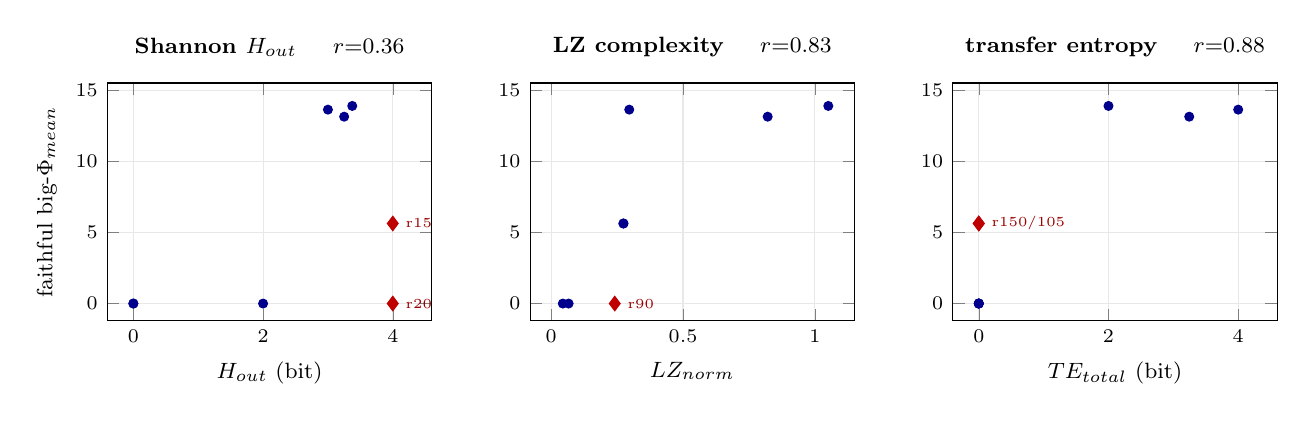
\begin{tikzpicture}
\begin{groupplot}[
  group style={group size=3 by 1, horizontal sep=1.25cm},
  width=5.7cm, height=4.6cm,
  ylabel near ticks, xlabel near ticks,
  ymin=-1.2, ymax=15.5,
  tick label style={font=\scriptsize},
  label style={font=\footnotesize},
  title style={font=\footnotesize\bfseries},
  grid=both, grid style={gray!18},
  scatter/use mapped color={draw=black,fill=blue!55!black},
]
% ---- panel 1: Shannon entropy (orthogonal) ----
\nextgroupplot[title={Shannon $H_{out}$ \quad $r{=}0.36$},
  xlabel={$H_{out}$ (bit)}, ylabel={faithful big-$\Phi_{mean}$}, xmin=-0.4, xmax=4.6]
\addplot[only marks, mark=*, mark size=1.6pt, blue!55!black]
  coordinates {(0,0)(0,0)(2,0)(3,13.625)(3.25,13.13)(3.375,13.885)};
\addplot[only marks, mark=diamond*, mark size=2.6pt, red!75!black]
  coordinates {(4,0)(4,5.625)};   % r204 max-H/zero-Phi, r150 max-Phi
\node[font=\tiny,red!60!black,anchor=west] at (axis cs:4,0)     {\,r204};
\node[font=\tiny,red!60!black,anchor=west] at (axis cs:4,5.625) {\,r150};
% ---- panel 2: LZ complexity (aligned) ----
\nextgroupplot[title={LZ complexity \quad $r{=}0.83$},
  xlabel={$LZ_{norm}$}, xmin=-0.08, xmax=1.15]
\addplot[only marks, mark=*, mark size=1.6pt, blue!55!black]
  coordinates {(0.044,0)(0.066,0)(0.274,5.625)(0.274,5.625)(0.296,13.625)(0.821,13.13)(1.051,13.885)};
\addplot[only marks, mark=diamond*, mark size=2.6pt, red!75!black]
  coordinates {(0.241,0)};   % r90 self-similar over-prediction
\node[font=\tiny,red!60!black,anchor=west] at (axis cs:0.241,0) {\,r90};
% ---- panel 3: transfer entropy (aligned) ----
\nextgroupplot[title={transfer entropy \quad $r{=}0.88$},
  xlabel={$TE_{total}$ (bit)}, xmin=-0.4, xmax=4.6]
\addplot[only marks, mark=*, mark size=1.6pt, blue!55!black]
  coordinates {(0,0)(0,0)(0,0)(0,0)(2,13.885)(3.245,13.13)(4,13.625)};
\addplot[only marks, mark=diamond*, mark size=2.6pt, red!75!black]
  coordinates {(0,5.625)(0,5.625)};   % r150/r105 XOR synergy blind spot
\node[font=\tiny,red!60!black,anchor=west] at (axis cs:0,5.625) {\,r150/105};
\end{groupplot}
\end{tikzpicture}
\caption{Faithful IIT~4.0 big-\bigphi{} vs.\ three classical information
measures on the identical ten-rule ECA panel (blue dots; red diamonds mark
the diagnostic dissociations). \textbf{Left:} Shannon output entropy ---
orthogonal (\(r=0.36\)); at \(H=\SI{4}{bit}\), \bigphi{} spans \(0\)
(identity~204) to \(5.6\) (XOR~150). \textbf{Centre:} LZ complexity ---
aligned (\(r=0.83\)); rule~90 has non-trivial LZ yet \(\bigphi=0\), the
self-similar over-prediction. \textbf{Right:} transfer entropy --- aligned
(\(r=0.88\)); XOR rules 150/105 sit at TE\(=0\) yet \(\bigphi=5.6\), the
synergy blind spot. Each classical measure has a blind spot \bigphi{} does
not.}
\label{fig:headline}
\end{figure}

\begin{table}[t]
\centering
\small
\begin{tabular}{lccl}
\toprule
\textbf{network} & \textbf{edges} & \(\bigphi_\mathrm{mean}\) & \textbf{note} \\
\midrule
scale-free hub (paw) & 4 & \(6.81\) & matched density \\
regular cycle (4-cyc) & 4 & \(0.00\) & matched density \\
empty & 0 & \(0.00\) & null anchor \\
complete (K$_4$) & 6 & \(5.625\) & integration ceiling \\
\bottomrule
\end{tabular}
\caption{Structure experiment (parity dynamics, \(N=4\)). At four edges,
the hub integrates where the cycle does not; the hub also exceeds the
denser complete graph. Topology, not edge count, governs \bigphi{}. The
cycle's zero is partly a parity-even-cycle decoupling confound
(\S\ref{sec:limits}).}
\label{tab:results}
\end{table}

\medskip
\noindent\textbf{Synthesis.} Reading the three correlations together
(Tab.~\ref{tab:panel}): \bigphi{} is orthogonal to the single-system
measure (Shannon entropy) and aligned with the inter-element measures (LZ,
transfer entropy). Neither aligned measure equals \bigphi{}: LZ
over-counts self-similarity, bivariate TE under-counts synergy. \bigphi{}
fills both gaps. The structure experiment closes the loop --- when only
the wiring is changed, \bigphi{} changes from \(0\) to \(6.8\). The
through-line is that \bigphi{} measures \emph{how elements relate}, which
is why no single classical scalar reproduces it, and why IIT posits it as
a distinct quantity.

\section{Discussion}
\label{sec:discussion}

\textbf{Why entropy dissociates but flow does not.} Shannon output
entropy is a property of a system's input--output map considered as a
single channel: a bijection is maximally informative regardless of
whether its cells interact. Integration, by construction, is a property
of the \emph{joint} cause--effect structure --- it asks what is lost when
the system is cut. The identity rule is the sharpest illustration: it is
a perfect channel (\(H=N\)) made of \(N\) independent perfect channels, so
cutting it loses nothing (\(\bigphi=0\)). Transfer entropy and LZ
complexity correlate with \bigphi{} precisely because they are sensitive
to inter-element dependence --- TE explicitly (directed conditional
dependence) and LZ implicitly (a space--time diagram is incompressible
only when distant cells co-determine each other). This is why the
single-system measure is orthogonal and the relational measures align.

\textbf{The two blind spots are complementary.} LZ \emph{over}-predicts on
rule~90: a Sierpi\'nski gasket is visually intricate and compresses
poorly under a one-dimensional LZ parse, yet the rule's cells are
pairwise-XOR with no irreducible whole, so \(\bigphi=0\). Bivariate TE
\emph{under}-predicts on rules~150/105: XOR-of-three is the canonical
synergistic gate, invisible to any pairwise conditional measure. A measure
can thus mistake pattern for integration (LZ) or miss integration hidden
in higher-order coupling (bivariate TE). \bigphi{}, computed over the full
cause--effect structure rather than a fixed-order statistic, is subject to
neither failure --- which is the operational content of IIT's claim that
\bigphi{} is a distinct quantity, not merely a third correlate.

\textbf{Relation to partial-information decomposition.} The TE blind spot
is exactly the synergy term in the Williams--Beer decomposition
\citep{williamsbeer2010}: pairwise TE captures unique and redundant
information flow but not synergy. A conditional / multivariate transfer
entropy (causation entropy) would recover the XOR rules and likely raise
the TE--\bigphi{} correlation above the reported \(r=0.88\); our bivariate
choice is the most conservative, and the fact that it already correlates
strongly is the point.

\textbf{Structure as the unifying axis.} The topology experiment
(\S\ref{sec:structure}) removes the dynamics-rule confound: holding edge
count fixed and changing only the wiring moves \bigphi{} from \(0\)
(cycle) to \(6.8\) (hub), and the hub exceeds the denser complete graph.
Read with the measure results, the through-line is that \bigphi{} is a
relational quantity --- it scores how a system's parts constrain one
another, which is why it tracks flow and complexity, ignores raw
information, and depends on wiring rather than density.

\section{Limitations and honest caveats}
\label{sec:limits}

\begin{itemize}\itemsep0.25em
\item \textbf{Small \(N\).} Exact big-\bigphi{} is computed at \(N=4\);
absolute \(r\) values depend on the ten-rule panel composition. The
directions (orthogonal vs.\ aligned) are robust to panel choice; the exact
coefficients are not.
\item \textbf{One estimator each.} Output-image entropy, single-seed LZ76,
and lag-1 \emph{bivariate} TE are one choice each. The XOR synergy blind
spot (\S\ref{sec:te}) is specifically a property of \emph{bivariate} TE;
a multivariate variant recovers it (\S\ref{sec:teorder}) but, as measured,
trades it for an opposite over-prediction rather than improving the fit.
Endpoints (constant\(=\)low, bijection\(=\)max entropy) are
definition-robust; mid-range magnitudes are not.
\item \textbf{State-averaged \bigphi{}.} Faithful \bigphi{} is
state-dependent; we average over states, so directions are trusted and
absolute magnitudes are hedged.
\item \textbf{Structure confound.} The cycle's \(\bigphi=0\)
(\S\ref{sec:structure}) is partly a parity-on-even-cycle decoupling
artifact, and a cycle is not a random ER graph; the robust claim is the
weak form (topology not density), and a clean ER ensemble needs
\(N\ge5\) (engine cost; deferred).
\item \textbf{Structure-cut, not absolute PyPhi calibration.} The engine
computes a spirit-faithful structure-cut big-\bigphi{}; absolute-scale
comparison to reference IIT implementations is out of scope. Our
conclusions are about \emph{correlation presence/absence} and are robust
to a scale offset.
\item \textbf{No phenomenal claim.} ECA rules are substrate proxies. ``XOR
integration,'' ``life-themed,'' etc.\ are structural labels, not claims
about phenomenal consciousness. The result is a measurement fact, not a
metaphysics.
\end{itemize}

\section{Future work}
\label{sec:future}

Four follow-ups are pre-specified. \emph{(i) Decompose the flow.} The
multivariate result (\S\ref{sec:teorder}) showed that recovering synergy
does not improve the \bigphi{}-correlation, because it over-counts
non-integrated flow (rule~90); a partial-information decomposition would
separate the synergy, redundancy, and unique terms and test each against
\bigphi{} individually, isolating which flow component (if any) tracks
integration. \emph{(ii) Larger panels and \(N\).} The exact engine is tractable
to \(N\!\approx\!8\); a 256-rule sweep and an \(N\ge5\) run would turn the
ten-point correlations into distributions and let the structure
experiment use a genuine Erd\H{o}s--R\'enyi ensemble, removing the
parity-even-cycle confound of \S\ref{sec:structure}. \emph{(iii)
Self-reference.} A companion experiment in this lane finds that closing a
self-loop creates or destroys a self-consistent fixed point depending on
base topology --- an ``\(I\)-as-fixed-point'' result that extends the
relational reading of \bigphi{} to self-modelling substrates. \emph{(iv)
Beyond toy substrates.} The same three-measure triangulation can be run on
small biological or artificial recurrent networks where an approximate
\bigphi{} is computable, testing whether the entropy-orthogonality and the
two blind spots survive outside cellular automata.

\section{Reproducibility}
\label{sec:repro}

Code: \url{https://github.com/dancinlab/anima} (hypotheses
\texttt{H\_287}--\texttt{H\_290} plus the multivariate-TE follow-up
\texttt{H\_293} under \texttt{UNIVERSE/}, with smoke sources and
\texttt{run.log} per experiment). Data: \texttt{companion/}
(\texttt{verify-ledger.json} carries every panel value, Pearson/Spearman
coefficient, pre-registered falsifier and its pass/fail;
\texttt{pr-roll.json} the landing PRs \#582--585;
\texttt{session-journal.md} the build narrative). Engine: the faithful
IIT~4.0 cause--effect library is reused, not reinvented (no new engine
code). All experiments: deterministic, \$0, CPU-only, no GPU, no language
model; re-run bit-for-bit identical. Build: \texttt{make} (xelatex
\(\times 3\) + bibtex). Figures: \texttt{make figures}.

\paragraph{Acknowledgments.}
Experiments were designed, run, and written up in a single foreground
session with an LLM collaborator (Claude); all numeric results are
deterministic outputs of the cited hexa-native smokes, independently
re-runnable without the model.

\appendix

\section{Pre-registered falsifier ledger}
\label{app:falsifiers}

Every experiment froze its falsifiers before the headline values were
read; each is reproduced from \texttt{companion/verify-ledger.json}. The
gate columns are measurement-validity checks (anchors, bounds,
determinism); the \emph{verdict} row is the hypothesis outcome, which for
H\_287 is an intended falsification (the closed negative). Notably no
falsifier was edited after the fact: H\_289's robustness falsifier and the
structure confound are reported as found.

\begin{table}[h]
\centering
\small
\begin{tabular}{llcl}
\toprule
\textbf{Exp.} & \textbf{measure / axis} & \textbf{gate} & \textbf{hypothesis verdict} \\
\midrule
H\_287 & Shannon entropy   & 11/11 & \tierRed{} \(r=0.363<0.5\) (reductive falsified) \\
H\_288 & LZ complexity     & 9/9   & \tierGreen{} \(r=0.831\), \(\rho=0.936\) \\
H\_290 & transfer entropy  & 8/8   & \tierGreen{} \(r=0.883\), \(\rho=0.822\) \\
H\_289 & network topology  & 4/4   & \tierGreen{} hub \(6.81>\) cycle \(0\) (confound-flagged) \\
H\_293 & multivariate TE   & 8/8   & \tierYellow{} synergy recovered, \(r\) drops \(0.883\!\to\!0.705\) (no TE order \(=\bigphi\)) \\
\bottomrule
\end{tabular}
\caption{Per-experiment gate counts and frozen-falsifier verdicts. Engine
anchors (rule~204, rule~0 \(\to\bigphi{=}0\)) are reproduced to machine
precision in all four; all four re-run bit-for-bit identically.}
\label{tab:falsifiers}
\end{table}

\section{Engine anchors}
\label{app:anchors}

The faithful IIT~4.0 engine is validated, before any correlation is read,
against two states whose \bigphi{} is hand-derivable. Rule~204 maps each
cell to its own current value (\(\mathrm{next}_i=c\)); the system is a
direct product of \(N\) one-cell mechanisms, so the system cut is
reducible and \(\bigphi=0\) at every state. Rule~0 maps every state to the
all-zero state; with no state-dependence there is no integrated cause and
\(\bigphi=0\). The engine reproduces both to machine precision. Because
the panel additionally contains a max-entropy/zero-\bigphi{} rule (204),
a positive-\bigphi{}/zero-TE rule (150), and a non-trivial-LZ/zero-\bigphi{}
rule (90), the dissociations of \S\ref{sec:results} are anchored on
independently checkable points rather than on the fitted correlation
alone.

\bibliographystyle{plainnat}
\bibliography{references}

\end{document}
